\section{Cloud Computing}

Im folgenden Unterkapitel werden die Grundlagen und eine Definition des Cloud Computing erarbeitet um den Kontext dieser Arbeit herleiten zu können.
Hierbei wird vorallem auf die Definition des Cloud Computing nach dem NIST und einiger Grundlagen nach Reinheimer2018 eingegangen.

\subsection{Was ist Cloud Computing}

Cloud Computing ist ein Modell der Zurverfügungstellung eines universell erreichbaren,
günstigen Netzwerkzugangs zu einer Ansammlung konfigurierbarer Computing Ressourcen
(z.B. Netzwerke, Server, Speicher, Anwendungen und Services), die mit minimalem Managementaufwand schnell freigegeben und bereitgestellt werden können
\cite[Vgl.][S. 2]{Mell2011}.

\begin{wrapfigure}{r}{0.45\textwidth}
\centering
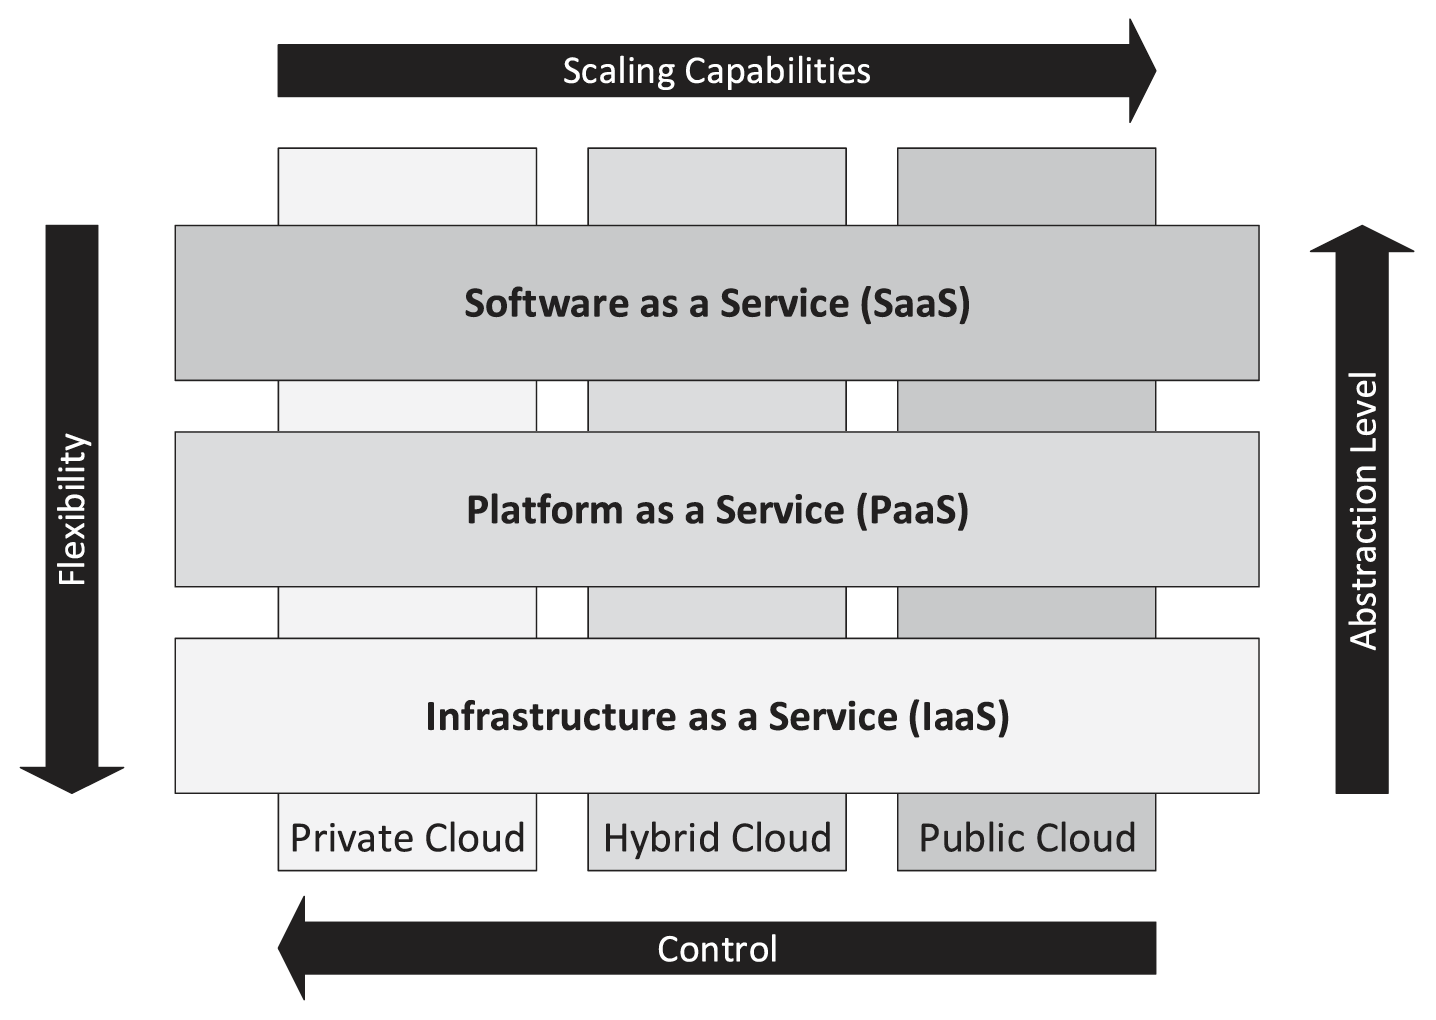
\includegraphics[height=0.3\textwidth]{xaas_maenhaut.png}
\caption{Eine Übersicht der Cloud Service Modelle \cite[S. 33]{Maenhaut2016}}
\label{fig:XaaS}
\end{wrapfigure}

Nach Hentschel und Leyh (2018) kann man Cloud Services grundsätzlich in drei Abstraktionsebenen einteilen. Diese sind \textbf{\acf{SaaS}},
\textbf{\acf{PaaS}} und \textbf{\acf{IaaS}}, welche auch zu \acf{XaaS} zusammengefasst werden
\cite[Vgl.][S. 9]{Reinheimer2018}.

Die unterste der drei genannten Abstraktionsschichten ist die \ac{IaaS}, welche die Basisinfrastruktur, wie zum Beispiel Netzwerk, Server oder Speicher,
bereitstellt. Diese Infrastruktur kann sowohl physisch als auch virtuell zur Verfügung gestellt werden \cite[Vgl.][S. 9f]{Reinheimer2018}.
Die darüberliegende Schicht ist die \ac{PaaS}, welche auf der Infrastruktur zusätzlich noch eine Basis zur Anwendungsentwicklung bietet, indem zum Beispiel
bereits ein Betriebssystem und eine Datenbank installiert sind oder eine andere Programmierumgebung verwendet werden kann \cite[Vgl.][S. 10]{Reinheimer2018}.
Die darüberliegende Schicht ist die \ac{SaaS}, welche standardisierte Anwendungen zur Verfügung stellt und sich somit direkt an den Endnutzer richtet
\cite[Vgl.][S. 11]{Reinheimer2018}.

In Abbildung \ref{fig:XaaS} wird eine Übersicht der drei Abstraktionsebenen angezeigt und dargestellt, wie es sich mit der Flexibilität über die verschiedenen
Service Level verhält \cite[Vgl.][S. 33]{Maenhaut2016}.

Generell wird die Cloud darüber hinaus in drei Organisationsdimensionen eingeteilt \cite[Vgl.][S. 7ff]{Reinheimer2018}:
\begin{itemize}
\item \textbf{Private Cloud:} In der Private Cloud haben nur bestimmte Nutzer Zugang zu der darunterliegenden Infrastruktur. Der Zugang wird meist mittels
\acf{VPN} ermöglicht. Die IT-Infrastruktur einer Private Cloud kann entweder im Unternehmenseigenen Rechenzentrum untergebracht oder auch
von Dienstleistern bereitgestellt werden.
\item \textbf{Public Cloud:} In der Public Cloud ist die Infrastruktur für mehr Anwender zugänglich und muss geteilt werden. Dafür muss als Anwender oft
auch nur für die tatsächlich genutzte Leistung gezahlt werden. Da die Infrastutktur jedoch gleichzeitig von vielen genutzt wird, ist zum Beispiel der
Betrieb von sicherheitskritischen Anwendungen schwierig.
\item \textbf{Hybrid Cloud:} Die Hybrid Cloud bildet eine kombinierte Anwendung aus der Public Cloud und der Private Cloud. Diese bietet dem Anwender die
Möglichkeit gewisse Anwendungen in die Public Cloud auszulagern, ohne die Vorteile der Private Cloud für sicherheitsrelevante Anwendungen aufgeben zu msüssen.
Darüber hinaus kann bei einem Hybrid Cloud modell die Rechenleistung der Private Cloud bei Spitzenlast durch die Public Cloud erweitert werden. 
\end{itemize}

\pagebreak

\subsection{Entwicklung des Cloud Computing}

Die Entwicklung des Cloud Computing und dessen Vorgängerkonzepte is bis in die 90er Jahre zurückzuführen.
Ein von Hentschel und Leyh (2018) hervorgehobender Vorgänger ist das sogrnannte Grid Computing.
Damit war bereits eine dezentrale Ressourcenkontrolle mir standardisierten Protokollen und
Schnittstellen realisiert. Das Cloud Computing bietet vergleichbare Eigenschaften, jedoch rückt der
Fokus hier auf wirtschaftliche Kriterien und die Zenralisierung von Ressourcen zum Beispiel in
Rechenzentren \cite[Vgl.][S. 5f]{Reinheimer2018}.

Nach Srivastava et al. (2018) war Salesforces eines der ersten Unternehmen, welches 1999 Anwendungen über eine Webseite bereitgestellt hat,
gefolgt von den \acf{AWS} in 2002, welche Speicher und Rechenleistung als Services bereitstellten \cite[Vgl.][S. 17f]{Srivastava2018}.

Durch die Entwicklungen im Cloud Computing haben sich drei Basiskomponenten herauskristallisiert \cite[Vgl.][S. 18]{Srivastava2018}:
\begin{itemize}
\item \textbf{Client Computer:} Über die Engeräte kann der Nutzer mit den Services der Cloud interagieren.
\item \textbf{Verteilte Server:} Die Server können verteilt über viele Orte stehen, funktionieren jedoch, wie ein zusammenhängendes System.
\item \textbf{Rechenzentren:} Die Rechenzentren bilden den Knotenpunkt für alle Server und beinhalten selbst weitere Server.
\end{itemize}

\pagebreak

\subsection{Herausforderungen -> Migration von Legacy Anwendungen}

Aus der vorangehend erläuterten Entwicklung des Cloud Computing ergeben sich verschiedene Herausforderungen.
Darunter fällt unter anderem die Migration von Legacy Anwendungen zu Cloud Anwendungen, welche gegeben durch die verschiedenen Service Level
auf unterschiedlichen Wegen realisiert werden kann.